% arara: pdflatex: { synctex: yes }
% arara: makeindex: { style: ctuthesis }
%% arara: bibtex

%\listfiles


%\PassOptionsToPackage{cp1250}{inputenc}

% The class takes all the key=value arguments that \ctusetup does,
% and couple more: draft and oneside
\documentclass[oneside]{ctuthesis}

\makeatletter
\edef\mytoday{\expandafter\@gobbletwo\the\year\ifnum\month<10 0\fi\the\month\ifnum\day<10 0\fi\the\day}
\makeatother

% LaTeX logo with better kerning in sf bf font
\makeatletter
\newcommand\LaTeX@lmss@bx{L\kern -.33em{\sbox \z@ T\vbox to\ht \z@ {\hbox {\check@mathfonts \fontsize \sf@size \z@ \math@fontsfalse \selectfont A}\vss }}\kern -.15em\TeX}
\DeclareRobustCommand\myLaTeX{%
	\ifcsname LaTeX@\f@family @\f@series\endcsname
		\csname LaTeX@\f@family @\f@series\endcsname
	\else
		\LaTeX
	\fi
}


\ctusetup{
	mainlanguage = english,
	secondlanguage = czech,
	otherlanguages = {czech},
%   title-czech = {Bias Detection in Czech News},
	title-english = {Bias Detection in Czech News},
	doctype = B,
	faculty = F3,
	department-czech = {Katedra počítačů},
	department-english = {Department of Computer Science},
	author = {Tomáš Horych},
	supervisor = {Ing. Jan Drchal, Ph.D},
	fieldofstudy-english = {Open Informatics},
	subfieldofstudy-english = {Artificial Intelligence and Computer Science},
	fieldofstudy-czech = {Matematcké inženýrství},
	subfieldofstudy-czech = {Matematické modelování},
	keywords-czech = {bias detekce, transformers, text classification},
	keywords-english = {bias detection, transformers, text classification},
	day = 10,
	month = 2,
	year = 2022,
	specification-file = {zadani.pdf},
    pkg-listings = true,
    ctulstbg = none,
}

\ctuprocess

% Theorem declarations, this is the reasonable default, anybody can do what they wish.
% If you prefer theorems in italics rather than slanted, use \theoremstyle{plainit}
\theoremstyle{plain}
\newtheorem{theorem}{Theorem}[chapter]
\newtheorem{corollary}[theorem]{Corollary}
\newtheorem{lemma}[theorem]{Lemma}
\newtheorem{proposition}[theorem]{Proposition}

\theoremstyle{definition}
\newtheorem{definition}[theorem]{Definition}
\newtheorem{example}[theorem]{Example}
\newtheorem{conjecture}[theorem]{Conjecture}

\theoremstyle{note}
\newtheorem*{remark*}{Remark}
\newtheorem{remark}[theorem]{Remark}

% Marginpars used as navigation aids.
\usepackage{mparhack}

\newcommand\indexmp[1]{{\sffamily\bfseries#1}}

\ExplSyntaxOn
\cs_new:Nn \ctuman_domarginpar:n {
	\marginpar
	[ \raggedleft \footnotesize \sffamily #1 ]
	{ \raggedright \footnotesize \sffamily #1 }
}
\cs_generate_variant:Nn \ctuman_domarginpar:n { x }
\DeclareDocumentCommand \ctump { m } {
	\clist_set:Nn \ctuman_temp_clist { #1 }
	\ctuman_domarginpar:x { \clist_use:Nnnn \ctuman_temp_clist { \\ } { \\ } { \\ } }
	\clist_map_inline:Nn \ctuman_temp_clist { \index{##1|indexmp} }
	\ignorespaces
}
\ExplSyntaxOff

% Abstract in Czech
\begin{abstract-czech}
Tento mánuál představuje \LaTeX ovou třídu ctuthesis, její použití, požadavky na systém atd.
\end{abstract-czech}

% Abstract in English
\begin{abstract-english}
This manual shows how to use the ctuthesis \LaTeX\ class, what are the requirements, etc.
\end{abstract-english}

% Acknowledgements / Podekovani
\begin{thanks}
We thank the CTU in Prague for being a~very good \emph{alma mater}.
\end{thanks}

% Declaration / Prohlaseni
\begin{declaration}
I declare that this work is all my own work and I have cited all sources I have
used in the bibliography.

\medskip

Prague, \monthinlanguage{title} \ctufield{day}, \ctufield{year}

\vspace*{2cm}

Prohlašuji, že jsem předloženou práci vypracoval samostatně, a že jsem uvedl veškerou použitou literaturu.

\medskip

V Praze, \ctufield{day}.~\monthinlanguage{second}~\ctufield{year}
\end{declaration}

\usepackage{url}
\usepackage{tabularx,array}
\usepackage{mathtools,amssymb}

% A savebox for typesetting listings in the titles
\newsavebox{\myboxa}

%\newcommand*\symbO{$\color{red}\bowtie$}
\newcommand*\symbO{\raisebox{0.5\height}{\scalebox{0.7}{\color{red}${\vartriangleright}\mkern-6mu{\vartriangleleft}$}}}
\newcommand*\symbM{\raisebox{0.5\height}{\scalebox{0.7}{\color{red}${\blacktriangleright}\mkern-6mu{\blacktriangleleft}$}}}
\newcommand*\itemO{\item\leavevmode\kern-0.33em\symbO}
\newcommand*\itemM{\item\leavevmode\kern-0.33em\symbM}



\begin{document}

% We actually don't want inline listings to have a background color
\renewcommand \ctulstsep {0pt}

% \ctuclsname for typesetting the class' name
\newcommand\ctuclsname{\leavevmode\unhcopy\ctuclsnamebox}
\newsavebox\ctuclsnamebox
\begin{lrbox}{\ctuclsnamebox}
\ctulst!ctuthesis!
\end{lrbox}

% all the formal stuff (abstract, title page etc)
\maketitle

















%-------------------------------------------------------------------------------------------------------------------
% MAIN TEXT
\chapter{Introduction}
This is introduction to my thesis, motivation. taky něco o nlp
\section{Motivation}
tady něco o nlp
\section{Outline}



\part{Data}
\chapter{Datasets} \label{datasets}
Due to the complex nature of bias, different datasets try to capture different aspects of it. In this section, I present a collection of \textbf{all} datasets related to biased writing and subjectivity detection available and later leveraged their bias information to augment smaller ground truth datasets. For details see experiment section \ref{experiments}.

As stated before, this work only focuses on sentence level classification, thus article level data were not considered.

\section{Subjectivity Datasets}

\subsection{SUBJ}
It is reasonable to include datasets that focus on the detection of subjectivity, since it's one of the media bias features. The Subjectivity dataset (SUBJ) \cite{Pang+Lee:04a} consists of 10000 sentences gathered from movie review sites. Sentences are labeled as subjective and objective with 1:1 ratio. 

The data were collected in an automatic way. The authors made an assumption that all reviews from Rottentomatoes\footnote{https://www.rottentomatoes.com/} are subjective and all plot summaries from IMBD\footnote{ www.imdb.com} are objective. Thus, the labels can be assumed to be noisy. For each class, 5k sentences were sampled \textbf{randomly}.




\subsection{MPQA}
\textbf{M}ulti-\textbf{P}erspective \textbf{Q}uestion \textbf{A}nswering (MPQA) Opinion corpus is another dataset that can be used for subjectivity detection. I used the MPQA Opinion corpus version 2.0, which consists of 692 articles from 187 different news sources summing up to 15802 sentences. All articles are from June 2001 to May 2002.

The corpus offers a rich annotation scheme \cite{wiebe2005annotating} that focuses on sentiment and subjectivity annotations.
\newpage
To extract the bias information, I focused on two types of annotations:
\begin{itemize}
    \item Direct subjective
    \item Expressive subjective
\end{itemize}
Which were present if any form of subjectivity was suspected by the annotator. Each annotation consists of indices of span in the text and properties. For each sentence in corpus I extracted labels as follows:

If there was at least one annotation \textbf{direct\_subjective} or \textbf{expressive\_subjectivity} with span inside the sentence and the intensity tag was not $low$, the sentence was labelled as \textit{subjective $\sim$ biased}. All other sentences were extracted as \textit{objective $\sim$ unbiased}.

This approach has yielded $9484$ subjective sentences and 6318 objective sentences.


\section{Media Bias datasets}


\subsection{BASIL}
BASIL dataset \cite{fan2019plain} comprises 300 articles with 1727 sentence level bias annotations. The authors of the dataset distinguish between \textbf{lexical} and \textbf{informational} bias.

The annotations were performed by two experts and further resolution discussions have later led to 0.56 and 0.7 \Gls{iaa} score for lexical and informational bias, respectively.

Even though BASIL brings the sufficient annotation quality, most of the labelling resulted in informational bias annotations, leaving only 478 sentences for the lexical bias class. Informational bias requires a different approach to detection \cite{van2020context} and usually depends on context dramatically. Therefore, I extracted all sentences with informational label as a neutral class.




\subsection{Ukraine Crisis Dataset}
This dataset \cite{farber2020multidimensional} offers 2057 sentences with binary media bias labels. All sentences are related to one topic - Ukraine-Russian crisis and data were gathered from 90 news sources.

The authors introduce rich annotations for each sentence. Each one of them looks at the bias from a different perspective, so called \textit{bias dimensions}:
\begin{enumerate}
    \item Hidden Assumptions and Premises
    \item Subjectivity
    \item Framing
\end{enumerate}
In addition, the \textit{overall bias} annotation is presented. Together, the data involve 44547 fine-grained annotations. For simplicity, I only included the overall bias annotation.
Even though this dataset encompasses comprehensive bias information, it also suffers from low \Gls{iaa} score. Specifically Krippendorff’s $\alpha = -0.05$.



\subsection{NFNJ}
The NFNJ\footnote{\cite{farber2020multidimensional} refer to this dataset as NFNJ, however in the original paper the name is not presented.} dataset provides 966 sentences from 46 articles with annotations on a fine-grained level.

Authors share the dataset for research purposes, however, the public version differs from the one described in the original paper. Therefore, while extracting the final dataset, I made a few assumptions:

In the raw data, contributions from multiple annotators on each sentence are provided. Therefore, I extracted the labels as a simple arithmetical mean of the labels. Furthermore, the original labels stand for 
\begin{itemize}
    \item 1: 'neutral'
    \item 2: 'slightly biased but acceptable'
    \item 3: 'biased'
    \item 4: 'very biased'
\end{itemize}
To obtain the final truth labels in a unbiased/biased format, I simply assumed sentences with mean-score $\leq$ 2 as neutral and $>$ 2 as biased.

The Fleiss Kappa \Gls{iaa} score averaged at zero, which makes it practically unusable as a standalone dataset.



\subsection{BABE}
\textbf{B}ias \textbf{A}nnotations \textbf{B}y \textbf{E}xperts (BABE) is a key media bias dataset from \Gls{mbg}\footnote{\url{https://media-bias-research.org/}}, which is to the best of my knowledge, the highest quality media bias dataset to this day. It builds on top of MBIC \cite{Spinde2021MBIC} which is a smaller crowdsourced dataset.

BABE contains 3700 sentences. 1700 sentences are from MBIC, which were extracted from 1000 news articles, and in addition extended by 2000 more sentences, altogether covering 12 topics, annotated with binary bias indications. In addition, the annotations were enriched with a list of biased words. However, the presence of biased words does not always result in an overall biased sentence label. See \ref{table:2} for examples.

It has been annotated by 8 experts resulting in \gls{iaa} Krippendorfs $\alpha = 0.39$, which exceeds other media bias datasets by a significant margin. It also provides detailed information about the annotator background, making it a \textbf{reliable} source of information. The pipeline of the collection of BABE can be seen in \ref{fig:babe-data}.

This dataset plays a pivotal role in my approach to media bias detection and is selected as a target for tuning language models in chapter \ref{experiments}. Examples of BABE data points can be seen in 
\ref{table:2}

\begin{table}
\makebox[\textwidth][c]{
\begin{tabular}[\textwidth]{l|c}
\textbf{sentence} & \textbf{label} \\
\hline
\cellcolor{biased_clr} Americans \colorbox{biasedw_clr}{know} President Donald Trump is an \colorbox{biasedw_clr}{outrageous}, \colorbox{biasedw_clr}{scandal-ridden} character. & biased \\

\cellcolor{unbiased_clr} Biden said he would seek Muslims to serve in his administration. & unbiased \\

\cellcolor{biased_clr} Biden’s shift \colorbox{biasedw_clr}{radically} leftward reflects that of his party. & biased \\

\cellcolor{unbiased_clr} Anti-vaccine groups take \colorbox{biasedw_clr}{dangerous} online \colorbox{biasedw_clr}{harassment} into the real world. & unbiased \\

\end{tabular}
}
\caption{Example of biased and unbiased sentences from \textbf{BABE}}
\label{table:2}
\end{table}


\begin{figure}
  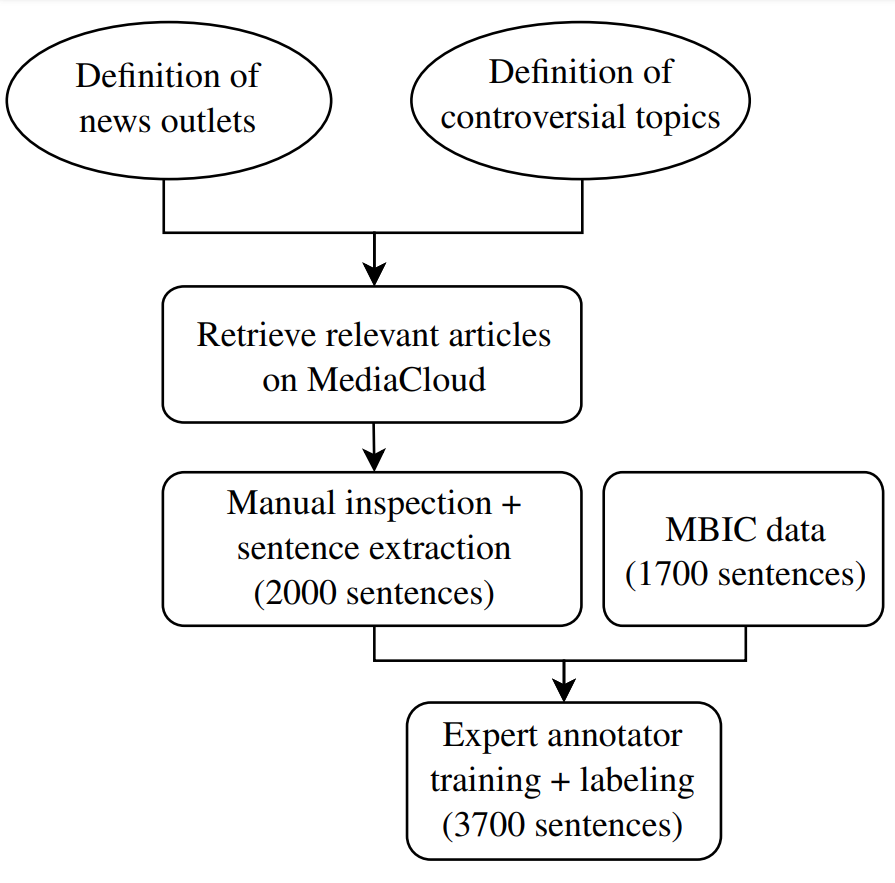
\includegraphics[scale=0.3]{my_modules/multimedia/babe_workflow.png}
  \caption{Data collection and annotation pipeline of \textbf{BABE}, reprinted from \cite{Spinde2021f}}
  \label{fig:babe-data}
\end{figure}



\section{Wikipedia NPOV datasets}\label{wiki-npov}
Due to annotation costs and the overall lack of large-scale datasets in the media bias setting, many researches \cite{pryzant2020automatically,recasens2013linguistic,hube2019neural} used Wikipedia's \Gls{npov} policy\footnote{\url{https://en.wikipedia.org/wiki/Wikipedia:Neutral_point_of_view}} to construct large-scale corpora automatically. 

Wikipedia's NPOV policy is a set of rules which aim to preserve neutrality in Wikipedia articles. Some examples of NPOV principles are:
\begin{itemize}
    \item Avoid stating opinions as facts.
    \item Avoid stating facts as opinions.
    \item Prefer nonjudgmental language.
\end{itemize}

When neutrality is contested, Wikipedia article can be moved to NPOV dispute by tagging it with \{\{NPOV\}\} or \{\{POV\}\}\footnote{Other POV related variations are ofthen used.} template. Debate on specific details of neutrality violations is then initialized among editors and eventually resolved, leading to removal of the tag.

This editorial information can be leveraged to extract parts of the text that violate NPOV and their unbiased counterparts. However, it has been shown \cite{hube2019neural,zhong-etal-2021-wikibias-detecting} that such automatic extraction can suffer from noisy labelling. In some cases \cite{hube2019neural} up to 60\% of data positive points were actually neutral.

Even though these datasets introduce a large amount of samples that are highly related to media bias, they are all sampled from Wikipedia's environment, which can be very different from the news environment. Effect of this domain gap on a training of a model is studied in \ref{experiments} section.




\subsection{Wiki Neutrality Corpus}\label{wiki}
\Gls{wnc} \cite{pryzant2020automatically} is a parallel corpus of 180k pairs of biased and unbiased sentences. For the collection of the data, \ref{wiki-npov} approach was adopted. The authors crawled revisions from 2014 - 2019. Each revision has been processed to check if it contains any variation of \textit{POV} related text in it. This approach yielded 180k pairs such that the sentence before edit is considered biased and the modified/added sentence after edit is considered neutral/unbiased.
    
In addition to WNC, 385k of sentences which have not been changed during the NPOV dispute were extracted as neutral and for word-level classification purposes, a subset of WNC corpus, where only one word is changed in the biased-unbiased pair, were added.




\subsection{CW-HARD}
Hube et al. \cite{hube2019neural} constructed a dataset based on NPOV, where only revisions with one sentence diff were filtered. However, because of the potentially noisy outcome, 5000 sentences were sampled and annotated using crouwdsourcing. Yet, the Krippendorffs Alpha agreement score measured only $\alpha = 0.124$ which is generally considered low. 

After filtering out sentences which annotators labeled with "I dont know" option, the final dataset consists of 1843 statements labeled as biased and 3109 labeled as neutral, a total of 4953 sentences.




\subsection{WikiBias}
This is the latest dataset based on Wikipedia. The authors \cite{zhong-etal-2021-wikibias-detecting} closely follow the approach of WNC \cite{pryzant2020automatically} and extract another parallel wiki corpus of 214k sentences.
To achieve a higher quality corpus, 4099 sentence pairs were randomly sampled and labeled by trained annotators. As a result, introduced \textbf{WikiBias-Manual} dataset consists of 3400 biased and 4798 neutral sentences annotated with high \gls{iaa} score of Cohen's $\kappa = 0.734$

\begin{table}
\begin{ctucolortab}
\begin{tabular}{c|c|c|c}
 \textbf{Dataset} & \textbf{Size} & \textbf{Annotation} & \textbf{Agreement}\\
 \hline
 \textbf{SUBJ} & 10.000 & automatic & -\\ 
 \hline
 \textbf{MPQA} & 15.802 & annotators & high \\
 \hline
 \textbf{BASIL} &  1.727 & annotators & medium \\ 
 \hline
 \textbf{Ukraine Crisis Dataset} & 2.057 & crowdsourcing & low \\ 
 \hline
 \textbf{NFNJ} & 888 & crowdsourcing & low \\
 \hline
 \textbf{BABE} & 3673 & annotators & medium \\
 \hline 
 \textbf{WNC} & 362.990 & automatic & - \\
 \hline
 \textbf{CW-hard} & 4953 & crowdsourcing & low \\
 \hline 
 \textbf{WikiBias} & 8198 & annotators & high \\
 \hline
\end{tabular}
\end{ctucolortab}
\caption{Comparison of all bias related datasets collected}
\label{table:1}
\end{table}



\section{Unused datasets}
 Some datasets focus on a slightly different task, yet still carry potentially useful information. Such data can be useful in a Multi-Task setting \ref{mtl}. To name a few, which are focused on a detection of ideology:
\begin{itemize}
\item \textbf{NewsB} - 
Consists of labels capturing authors political ideology (liberal, conservative) Labeled through distant supervision.
\item \textbf{IBC} - Also focuses on ideology detection, however, it is not publicly available.
\end{itemize}


\section{Summary}
In the previous section, I introduced all resources that are potentially useful for media bias analysis and are publicly available. The overview of all datasets and its properties can be seen in figure \ref{table:1}.

BABE dataset is generally a good benchmark and its translated parallel version will be used for evaluation in this work. Combinations of different datasets merging are studied in \ref{experiments}. Unfortunately a lot of the data suffer from noisy labelling and low \gls{iaa} greatly. Hence, their usability is considerably limited.


\part{models}
\chapter{Experiments}

\section{Transformer architecture}
\section{Czech models}
\subsection{RobeCzech,Czert,FERNET}
\section{Training}
RobeCzech \cite{thorne2019fever2}
\section{Evaluation}


%\appendix

\printindex

\bibliographystyle{amsalpha}
\bibliography{mythesis/citation}

\end{document}